\section{Генериране на графа}

\paragraph*{} Решението на задачата може да се раздели на две независими части - генерирането на графа и обхождането му. Реализирани са два варианта за записване на графа - като списъци на съседство и като матрица на съседство.

\subsection{Списъци на съседство}

\paragraph*{} Списъците на съседство са в общия случай по-бързи за генериране и обработка и заемат по-малко памет от матрицата, но не позволяват много добро разпареляване при генерирането на неориентиран граф.

\paragraph*{Ориентиран граф} \verb|graph::AdjLists::gen_directed()|. За генерирането на ориентиран граф се използва следната стратегия. Графа се разделя на множество части, всяка с фиксиран размер от $k$ върха (k = 128) и $m * {k \over n}$ ребра. За всяка част се пуска задача в thread pool-а, като часта с върхове \textit{a..b} генерира ребра започващи от нея, т.е. ребра \textit{(c, v)}, $a <= c <= b$. Така всяка нишка работи върху отделна част от графа.

Този подход не генерира напълно случаен граф, защото всяка част ще има един и същ брой ребра. Една причина да се генерира на части, а не всеки връх по отделно (т.е. k=1) е за да се намали този ефект.

\paragraph*{} Има и втори вариант на алгоритъма - \verb|AdjLists::gen_directed_on_threads()|, където графа се разделя на $t$ на брой равни части - по една за всяка нишка. Това служи за сравнение между ръчно направено разпределяне и автоматичното разпределяне от библиотеката rayon. Има micro benchmark за това в директория benches/, разликата e, че rayon е константно с около 10\% по-бавен. Всички по-нататъшни резултати използват \verb|AdjLists::gen_directed()|.

\paragraph*{Неориентиран граф} \verb|graph::AdjLists::gen_undirected()|. Генерирането на неориентиран граф е по-сложна задача, защото за всяко добавено ребро \textit{(u, v)}, трябва да се добави и обратното ребро \textit{(v, u)}. Първата стъпка е да се генерират ребрата \textit{(u, v)} така, че \textit{u > v}. Използва се същия подход като при ориентирания граф, с разликата, че броят ребра, които се генерират за часта с върхове от $a$ до $b$ е $m * (b^2 - a^2) \over n^2$.

\paragraph*{} След това трябва да се добавят огледалните ребра. Идеята е да обходим вече генерираните ребра, и за всяко ребро \textit{(a, b)} да добавим реброто \textit{(b, a)}. Ако се опитаме да направим това паралелно трябва да се добави синхронизация, защото може да се срещнат две ребра \textit{(a, b)} и \textit{(c, b)} едновременно, при което се получава едновременно писане в вектора \textit{b}.

Изпробвани са няколко подхода, но най-бързо се оказа това да се направи последователно на една нишка, поне за размерите на графа с който е тествано.

\subsection{Матрица на съседство}

\paragraph*{} Матрицата на съседство е имплементирана чрез конкурентен битов вектор. За целта съм модифицирал структурата предоставяна от една външна библиотека, като съм опростил интерфейса и съм заменил операциите за четене и писане на битове с атомарни такива.

При матрицата разпареляването на алгоритъма е лесно и в двата случая.

\paragraph*{Ориентиран граф} \verb|graph::AdjMatrix::gen_directed()|. Разделяме задачата на подзадачи, като всяка подзадача генерира фиксиран брой ребра. Подзадачите се изпълняват едновременно от thread pool. Всяка подзадача генерира случайно ребро \textit{(u, v)} и го записва в матрицата и проверява дали вече съществува с една атомарна операция. Това продължава докато не се генерират 128 ребра.

\paragraph*{Неoриентиран граф} \verb|graph::AdjMatrix::gen_undirected()| Идеята е същата като при ориентирания, с изключението че се генерират само ребра за които \textit{u < v}. Нишката пробва да добави реброто \textit{(u, v)}. Ако това успее, то реброто \textit{(v, u)} също не съществува и никой друг няма да се опита да го добави, затова нишката го добавя и него.

\subsection{Резултати}

\paragraph*{} Резултати от измерване върху t5600. Алгоритмите са измерени с два различни входа - 200\_000 върха, 4\_000\_000 ребра и 200\_000 върха, 40\_000\_000 ребра.

В случая на матрица на съседство отчетеното време не включва времето за заделяне на матрицата, което е 2.5 - 3 секунди.

\paragraph*{Списъци на съседство - ориентиран граф}

\begin{center}
\begin{tabular}{ c | c c c | c c c | }
  нишки & време (200k/4m) & $S_p$ & $E_p$ & време (200k/40m) & $S_p$ & $E_p$ \\
  \hline
  1  & 0.389 сек & 1 & 1 & 5.106 сек & 1 & 1 \\
  2  & 0.212 сек & 1.83 & 0.91 & 2.696 сек & 1.89 & 0.94 \\
  3  & 0.196 сек & 1.98 & 0.66 & 2.002 сек & 2.55 & 0.85 \\
  4  & 0.134 сек & 2.90 & 0.72 & 1.431 сек & 3.56 & 0.89 \\
  6  & 0.123 сек & 3.15 & 0.52 & 1.159 сек & 4.40 & 0.73 \\
  8  & 0.113 сек & 3.44 & 0.43 & 0.925 сек & 5.52 & 0.69 \\
  10 & 0.116 сек & 3.33 & 0.33 & 0.891 сек & 5.73 & 0.57 \\
  12 & 0.118 сек & 3.29 & 0.27 & 0.805 сек & 6.33 & 0.52 \\
  14 & 0.115 сек & 3.37 & 0.24 & 0.788 сек & 6.47 & 0.46 \\
  16 & 0.114 сек & 3.41 & 0.21 & 0.788 сек & 6.47 & 0.40 \\
  20 & 0.106 сек & 3.65 & 0.18 & 0.836 сек & 6.10 & 0.30 \\
  24 & 0.112 сек & 3.46 & 0.14 & 0.834 сек & 6.11 & 0.25 \\
  28 & 0.116 сек & 3.33 & 0.11 & 0.844 сек & 6.04 & 0.21 \\
  32 & 0.125 сек & 3.11 & 0.09 & 0.878 сек & 5.81 & 0.18 \\
\end{tabular}
\end{center}

\paragraph*{Списъци на съседство - неориентиран граф}

\begin{center}
\begin{tabular}{ | c | c c c | c c c | }
  нишки & време (200k/4m) & $S_p$ & $E_p$ & време (200k/40m) & $S_p$ & $E_p$ \\
  \hline
  1 &  0.729 сек & 1 & 1 & 8.868 сек & 1 & 1 \\
  2 &  0.580 сек & 1.25 &  0.62 & 6.262 сек & 1.41 & 0.70 \\
  3 &  0.516 сек & 1.41 &  0.47 & 5.290 сек & 1.67 & 0.55 \\
  4 &  0.498 сек & 1.46 &  0.36 & 4.998 сек & 1.77 & 0.44 \\
  6 &  0.493 сек & 1.47 &  0.24 & 4.541 сек & 1.95 & 0.32 \\
  8 &  0.491 сек & 1.48 &  0.18 & 4.487 сек & 1.97 & 0.24 \\
  10 & 0.487 сек & 1.49 &  0.14 & 4.421 сек & 2.00 & 0.20 \\
  12 & 0.494 сек & 1.47 &  0.12 & 4.350 сек & 2.03 & 0.16 \\
  14 & 0.508 сек & 1.43 &  0.10 & 4.506 сек & 1.96 & 0.14 \\
  16 & 0.495 сек & 1.47 &  0.09 & 4.416 сек & 2.00 & 0.12 \\
  20 & 0.496 сек & 1.47 &  0.07 & 4.362 сек & 2.03 & 0.10 \\
  24 & 0.491 сек & 1.48 &  0.06 & 4.383 сек & 2.02 & 0.08 \\
  28 & 0.494 сек & 1.47 &  0.05 & 4.468 сек & 1.98 & 0.07 \\
  32 & 0.510 сек & 1.43 &  0.04 & 4.503 сек & 1.96 & 0.06 \\
\end{tabular}
\end{center}

\begin{figure}[H]
  \centering
  \begin{minipage}{.45\textwidth}
    \centering
    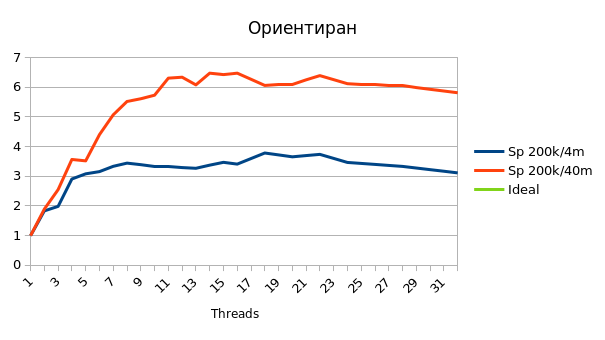
\includegraphics[width=\textwidth]{directed_lists.png}
  \end{minipage}
  \begin{minipage}{.45\textwidth}
    \centering
    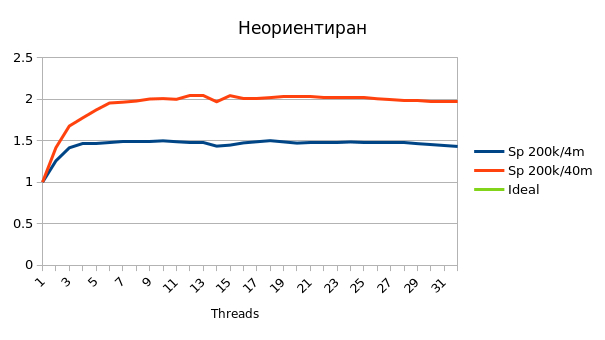
\includegraphics[width=\textwidth]{undirected_lists.png}
  \end{minipage}
\end{figure}

\paragraph*{Матрица на съседство - ориентиран граф}

\begin{center}
\begin{tabular}{ | c | c c c | c c c | }
  нишки & време (200k/4m) & $S_p$ & $E_p$ & време (200k/40m) & $S_p$ & $E_p$ \\
  \hline
  1  & 0.717 сек & 1 & 1 & 7.144 сек & 1 & 1 \\
  2  & 0.398 сек & 1.80 & 0.90 & 4.065 сек & 1.75 & 0.87 \\
  3  & 0.294 сек & 2.43 & 0.81 & 3.119 сек & 2.29 & 0.76 \\
  4  & 0.248 сек & 2.88 & 0.72 & 2.049 сек & 3.48 & 0.87 \\
  6  & 0.165 сек & 4.34 & 0.72 & 1.459 сек & 4.89 & 0.81 \\
  8  & 0.117 сек & 6.08 & 0.76 & 1.115 сек & 6.40 & 0.80 \\
  10 & 0.094 сек & 7.59 & 0.75 & 0.977 сек & 7.31 & 0.73 \\
  12 & 0.083 сек & 8.56 & 0.71 & 0.735 сек & 9.71 & 0.80 \\
  14 & 0.082 сек & 8.65 & 0.61 & 0.632 сек & 11.28 & 0.80 \\
  16 & 0.069 сек & 10.28 & 0.64 & 0.566 сек & 12.61 & 0.78 \\
  20 & 0.062 сек & 11.46 & 0.57 & 0.502 сек & 14.22 & 0.71 \\
  24 & 0.056 сек & 12.60 & 0.52 & 0.453 сек & 15.75 & 0.65 \\
  28 & 0.053 сек & 13.42 & 0.47 & 0.395 сек & 18.06 & 0.64 \\
  32 & 0.046 сек & 15.34 & 0.47 & 0.362 сек & 19.71 & 0.61 \\
\end{tabular}
\end{center}

\paragraph*{Матрица на съседство - неориентиран граф}

\begin{center}
\begin{tabular}{ | c | c c c | c c c | }
  нишки & време (200k/4m) & $S_p$ & $E_p$ & време (200k/40m) & $S_p$ & $E_p$ \\
  \hline
  1  & 0.943 сек & 1     & 1    & 9.443 сек & 1 & 1 \\
  2  & 0.514 сек & 1.83  & 0.91 & 5.196 сек & 1.81 & 0.90 \\
  3  & 0.439 сек & 2.14  & 0.71 & 4.326 сек & 2.18 & 0.72 \\
  4  & 0.292 сек & 3.22  & 0.80 & 2.698 сек & 3.49 & 0.87 \\
  6  & 0.213 сек & 4.41  & 0.73 & 1.920 сек & 4.91 & 0.81 \\
  8  & 0.151 сек & 6.23  & 0.77 & 1.392 сек & 6.77 & 0.84 \\
  10 & 0.144 сек & 6.52  & 0.65 & 1.192 сек & 7.91 & 0.79 \\
  12 & 0.119 сек & 7.86  & 0.65 & 1.133 сек & 8.33 & 0.69 \\
  14 & 0.105 сек & 8.93  & 0.63 & 0.841 сек & 11.22 & 0.80 \\
  16 & 0.090 сек & 10.37 & 0.64 & 0.758 сек & 12.45 & 0.77 \\
  20 & 0.088 сек & 10.68 & 0.53 & 0.707 сек & 13.35 & 0.66 \\
  24 & 0.080 сек & 11.70 & 0.48 & 0.694 сек & 13.60 & 0.56 \\
  28 & 0.072 сек & 12.92 & 0.46 & 0.679 сек & 13.90 & 0.49 \\
  32 & 0.072 сек & 12.97 & 0.40 & 0.610 сек & 15.45 & 0.48 \\
\end{tabular}
\end{center}

\begin{figure}[H]
  \centering
  \begin{minipage}{.45\textwidth}
    \centering
    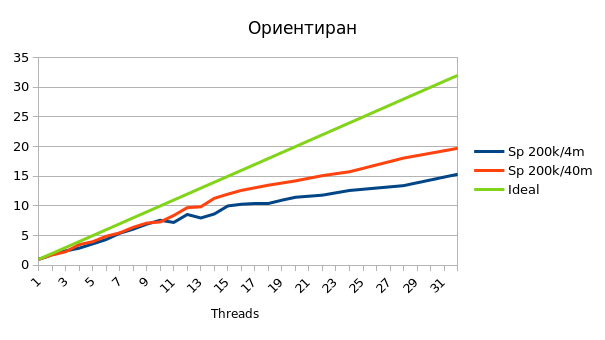
\includegraphics[width=\textwidth]{directed_matrix.png}
  \end{minipage}
  \begin{minipage}{.45\textwidth}
    \centering
    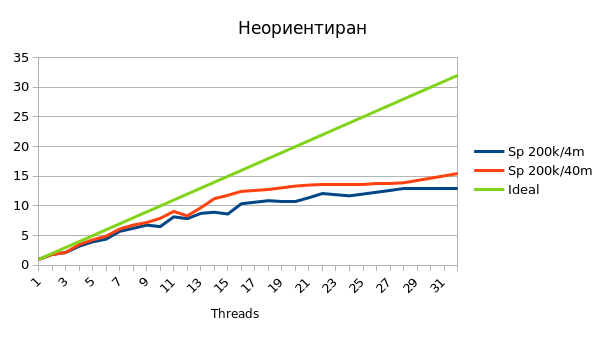
\includegraphics[width=\textwidth]{undirected_matrix.png}
  \end{minipage}
\end{figure}
